\section{Introduction}
Large Language Models (LLMs), such as GPT-4 and Claude, have achieved remarkable progress in natural language understanding and generation \cite{zhang2024supervised, ding2024hybrid, fang2024large}, driving advancements in fields ranging from conversational AI \cite{dam2024complete, dong2023towards} to content creation \cite{liang2024monitoring, shao2024assisting} and agentic task delegation \cite{guo2024embodied, agashe2023evaluating, xi2023rise}. LLMs are increasingly integrated into applications that influence everyday activities, such as planning, acting, and decision-making. Therefore, the ability of LLMs to navigate complex situations has significant implications for their deployment in applications requiring strategic interaction, such as automated negotiations, economic modeling, and collaborative problem-solving \cite{bianchi2024well, horton2023large, li2024econagent, chen2024comm, li2023metaagents}.

Despite the wide exploration and utilization, LLM's capacity for rational behavior, particularly in strategic settings represented by game theory, remains an open question \cite{leng2023llm, stade2024large, wu2024shall, de2023emergent, lan2023llm}. In this context, rationality implies an agent’s ability to make decisions that maximize expected utility based on available information, an essential component of intelligent and adaptive decision-making. In the realm of game theory, rational agents are expected to act strategically, considering not only their own preferences but also the potential actions and preferences of others. This is especially critical in incomplete-information games, where uncertainty about other players' information necessitates sophisticated reasoning and belief updating. 

This paper investigates the capacity of LLMs to behave rationally in game-theoretic scenarios and explores methodologies to enhance their rational decision-making capabilities. We begin by assessing the performance of several state-of-the-art LLMs, including Claude-3.5 Sonnet, Claude-3 Opus, GPT-4o and o1 \cite{zhong2024evaluation}, in both complete-information and incomplete-information games such as the Prisoner's Dilemma, Battle of the Sexes, the Escalation Game, and Deal-or-No-Deal \cite{lewis2017deal}, presented in Figure~\ref{fig:game_framework}. Our analysis reveals LLMs often deviate from rational strategies, particularly as the complexity of the game increases with larger payoff matrices or deeper sequential trees (Section \ref{sec:complete}). They also exhibit a lack of robustness to noise and uncertainty, leading to suboptimal outcomes (Section \ref{sec:observation}).

\textbf{To address these limitations, we introduce a novel approach by proposing game-theory-inspired workflows specifically designed to guide the reasoning and decision-making processes of LLMs. This is the first attempt to systematically integrate classic game-theoretic strategies into LLM-based agent workflow, aiming to enhance their rational behavior and decision-making capabilities in strategic settings.}
These workflows incorporate principles such as \textit{Dominant Strategy Search}, which involves identifying strategies that yield the highest payoff regardless of the opponent's actions; \textit{Backward Induction}, a method of solving extensive-form games by analyzing them from the end states backward to the initial decision nodes to determine optimal strategies; and \textit{Bayesian belief updating}, which allows agents to refine their beliefs about other players' valuations based on observed actions and signals during the game. Cringed on these well-defined and well-studied game-theoretic methods, we design algorithms to guide the behavior and thinking process of LLM-based agents.

Additionally, we integrate fairness considerations like envy freeness and pareto optimality, which promote equitable and efficient outcomes in negotiations by ensuring that no agent prefers another agent's allocation to their own and that no improvements can be made without making at least one agent worse off. 
%By embedding these mechanisms into the LLMs' reasoning processes, we aim to align their behavior more closely with that of rational agents as defined in game-theoretic terms.

\begin{minipage}[t]{1\linewidth} 
\begin{tcolorbox}[colback=gray!5,colframe=blue!40!black,title=Contribution Summary]
\begin{itemize}
    \item Comprehensive Evaluation of LLMs in Strategic Games and Identification of Rationality Limitations in LLMs (Section~\ref{sec:complete} and~\ref{sec:observation}): Through empirical analysis, we uncover that LLMs often fail to behave rationally in strategic settings, exhibiting a lack of robustness to noise and randomness. 
    \item Design of Game-Theory-Inspired Workflows (Section~\ref{sec:complete_workflow} and~\ref{sec:incomplete_workflow}): We develop novel workflows inspired by game-theoretic concepts to guide the reasoning and decision-making processes of LLMs, incorporating analysis and algorithms from classic game theory. 
    \item Emerging Research Direction (Section~\ref{sec:oneworkflow} and~\ref{sec:meta-strategy}): Through the application of workflows, we identify a promising new research direction in meta-strategy, specifically focusing on the decision of whether to adopt a workflow and, potentially, which workflow to employ in varying scenarios.
\end{itemize}
\end{tcolorbox} 
\end{minipage} 

\begin{figure}[!ht]
    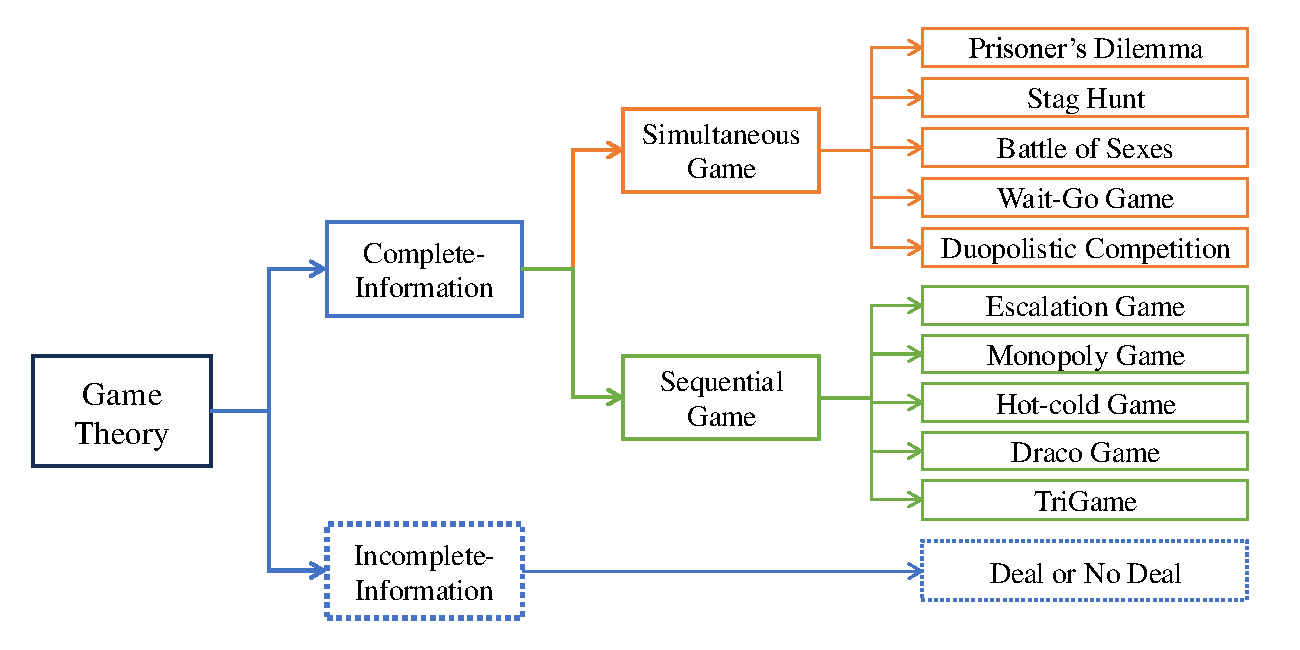
\includegraphics[scale=0.6]{Fig/framework.pdf}
    \caption{Game-theoretic Landscape Investigated in this Paper.}
    \label{fig:game_framework}
\end{figure}
